% =====================================================================
%  SECTION 4 — ALUMINIUM DOWNSTREAM INDUSTRY LOGIC
%
%  Segmentation derived from effective-protection theory (Corden 1966;
%  Balassa 1965, 1968), the report's own HS 7601--7616 scope, the ERP
%  basket in ERP.xlsx / Tariff FD.xlsx, and the OECD (2019) aluminium
%  value-chain segmentation:
%     UPSTREAM   = primary smelting, NIC 2420, output HS 7601--7603
%                  (the dutiable input)
%     DOWNSTREAM = conversion activities -- extrusion, rolling, drawing,
%                  casting, structural fabrication, utensils and other
%                  articles; NIC 2432 + 2511 + 2599, output HS 7604--7616
%                  (the thirteen ERP basket lines)
%
%  All figures regenerated from ASI_National.csv by asi_downstream_logic.py.
%  Full numeric output in asi_downstream_output.txt.
%
%  FIGURE DESIGN: every series is separated by THREE redundant cues --
%  line style, marker shape and marker fill -- so the figures remain
%  readable in black and white, photocopied or faxed. Legends sit above
%  the plotting area and never overlie data. Values are printed on the
%  plot so no number has to be read off an axis.
%
%  Requires the preamble of aluminium_report.tex (pgfplots, booktabs,
%  patterns, colours g1--g9, float [H]).
%  Requires \label{sec:scope} and \label{sec:erp}.
%  Requires bibitems: corden1966, balassa1965, balassa1968, cullen2013,
%  bertram2009, bohlin2006, millerblair (added by build_downstream_report.py).
% =====================================================================

% ---------- shared print-safe figure styles --------------------------
\pgfplotsset{
    asibase/.style={
        width=15cm,
        tick label style={font=\small},
        ymajorgrids=true, major grid style={black!12},
        axis line style={black!60},
        legend style={
            at={(0.5,1.03)}, anchor=south,
            draw=black!45, fill=white, font=\small,
            /tikz/every even column/.append style={column sep=10pt}},
        legend cell align={left},
        x tick label style={rotate=45, anchor=east, font=\scriptsize},
        % Opaque white chip behind every printed value, so a plot line or
        % gridline passing beneath can never merge with the digits.
        every node near coord/.append style={
            font=\tiny, black, fill=white, fill opacity=1, text opacity=1,
            inner sep=1.1pt, outer sep=0pt},
    },
}
% Series styles must live in the /tikz/ namespace: they are applied to \addplot.
% Three redundant cues per series -- line style, marker shape, marker fill --
% so that no series depends on colour or grey level to be identified.
\tikzset{
    upstyle/.style={black, thick, mark=*,       mark size=2.1pt, mark options={solid, fill=black}},
    dnstyle/.style={black, thick, dashed, mark=square*, mark size=2.1pt, mark options={solid, fill=white}},
    altA/.style={black!65, thick, densely dotted, mark=triangle*, mark size=2.6pt, mark options={solid, fill=black!20}},
    altB/.style={black, thick, dashdotted, mark=diamond*, mark size=2.6pt, mark options={solid, fill=white}},
    upbar/.style={fill=g2, draw=black, line width=0.5pt,
                  postaction={pattern=north east lines, pattern color=black!65}},
    dnbar/.style={fill=g8, draw=black, line width=0.5pt},
}

\section{Policy Plight of MSMEs in the Aluminium Industry}

\subsection{Measuring the Sector: Where the Value Chain Divides}
\label{sec:asi_method}

The claims made so far deserve to be tested against official statistics rather than industry assertion, and for that we use the \textbf{Annual Survey of Industries (ASI)} \cite{asi2024}. Everything then turns on where the chain is divided, and the division used here is not a matter of taste: it is the one the theory behind Section~\ref{sec:erp} requires.

Corden \cite{corden1966} defines the object of effective-protection analysis as an \emph{activity}---a stage of conversion from traded input to traded output, whose protection depends jointly on the tariff on that output and the tariffs on its inputs. The aluminium chain therefore divides where metal stops being something a producer makes and becomes something a producer buys. On one side stands the metal itself, \textbf{HS~7601--7603}, carrying the basic customs duty of 7.5 per cent. On the other stand all the activities that buy it at a duty-inclusive price and convert it---extrusion, rolling, wire drawing, foil, shape casting, structural fabrication, utensil manufacture. Each faces the same wedge between a protected input and an output whose own tariff has been bargained away, so on Corden's criterion they are one class of activity: precisely the thirteen lines \textbf{HS~7604--7616} on which Section~\ref{sec:erp} estimates effective protection.

The pathology has a precedent. Balassa found the effective rate on United States wool clothing turning \emph{negative} because wool yarn and fabric were themselves protected \cite{balassa1965}, and established tariff escalation as the systematic feature that penalises processing \cite{balassa1968}; Pathania and Bhattacharjea document the same result across Indian manufacturing \cite{pathania2020}. Industry practice draws the line in the same place: the OECD treats semi-fabrication as a \emph{downstream} activity and finds upstream support conferring advantage on it \cite{oecd2019}. The material-flow literature is finer-grained---Cullen and Allwood separate semi-fabrication from fabrication as distinct process steps \cite{cullen2013,bertram2009}---but a tariff does not distinguish a rolling mill from a window fabricator, and where the distinction might matter it is tested rather than assumed (Appendix~\ref{app:asi}).

Applying the rule yields the concordance in Table~\ref{tab:nic_concordance} \cite{nic2008}.

\begin{table}[H]
    \centering
    \caption{The thirteen ERP product lines mapped to their ASI manufacturing classes}
    \label{tab:nic_concordance}
    \resizebox{\textwidth}{!}{
    \begin{tabular}{llp{6.6cm}l}
        \toprule
        \textbf{HS line} & \textbf{Product} & \textbf{Converting activity} & \textbf{NIC class} \\
        \midrule
        \multicolumn{4}{l}{\textit{Upstream --- the dutiable input, not part of the ERP basket}} \\
        7601 & Unwrought aluminium & Smelting from alumina & \textbf{2420} \\
        7602 & Waste and scrap & Secondary refining & \textbf{2420} \\
        7603 & Powders and flakes & Atomising, milling & \textbf{2420} \\
        \midrule
        \multicolumn{4}{l}{\textit{Downstream --- the thirteen ERP basket lines}} \\
        7604 & Bars, rods, profiles & Extrusion & 2432 \\
        7605 & Wire & Wire drawing & 2432 \\
        7606 & Plates, sheets, strip & Flat rolling & 2432 \\
        7607 & Foil & Foil rolling & 2432 \\
        7608 & Tubes and pipes & Extrusion, drawing & 2432 \\
        7609 & Tube and pipe fittings & Fabrication, machining & 2599 \\
        7610 & Structures, doors, windows, fa\c{c}ades & Structural fabrication & \textbf{2511} \\
        7611 & Reservoirs, tanks, vats & Tank fabrication & \textit{2512} \\
        7612 & Casks, drums, cans & Container fabrication & 2599 \\
        7613 & Containers for compressed gas & Cylinder fabrication & \textit{2512} \\
        7614 & Stranded wire, cables, plaited bands & Stranding, plaiting & 2599 \\
        7615 & Table, kitchen and household articles & Utensil manufacture & \textbf{2599} \\
        7616 & Castings and other articles & Shape casting, general fabrication & \textbf{2432}, 2599 \\
        \bottomrule
    \end{tabular}
    }

    \vspace{0.2cm}
    \raggedright
    \small \textbf{Notes.} \textbf{Upstream $=$ NIC~2420; downstream $=$ NIC~2432 $+$ 2511 $+$ 2599.} NIC~0729 (bauxite) and NIC~2512 are not separately available in the ASI All-India summary. NIC~2710, 2732, 2733 and 3030 are excluded: their principal outputs fall in HS Chapters~85 and~88, which on Corden's criterion makes them a different activity, protected by a different set of tariffs. Appendix~\ref{app:asi} states the rule in full, together with the treatment of classes that are not exclusive to aluminium and the effect of every alternative tested.
\end{table}

Three things should be said before the evidence, each developed in Appendix~\ref{app:asi}. All values are nominal, at current prices. All stated statistics run to \textbf{2022--23}. And the comparison is biased \emph{against} our own conclusion: semi-fabrication carried out inside integrated smelters is recorded upstream, NIC~2512 is not separately published, and the ASI frame excludes the unincorporated units in which downstream fabrication is concentrated. All three inflate the measured upstream segment and deflate the downstream one, so every gap below is a lower bound.

\paragraph{What the evidence is, and is not.} What follows is association, not an identified causal effect. The data show that the class the effective-protection analysis identifies as most disprotected is also the class whose value added, employment and tax contribution have stagnated, and they supply a mechanism---an input-cost share of 83.1 per cent---by which the first could produce the second. There is no counterfactual India without the duty, the effective-protection series runs to three years against twelve of ASI data, and the construction cycle is not separately controlled for. What can be said is that the association holds in sign in every year of the record and is concentrated in precisely the class the tariff analysis singles out. A causal claim would require firm-level data spanning a tariff change; we do not make one.

\subsection{Value Added and Employment}

Over the eleven years to 2022--23 the two segments did not grow alike. Upstream gross value added rose \textbf{138.4 per cent} against \textbf{114.5 per cent} downstream, leaving them of comparable size---INR 42,662 crore against INR 41,653 crore---where downstream had begun the period the larger (Figure~\ref{fig:asi_index}). Measured between three-year averages at each end, which removes the sensitivity to a volatile base year, the gap is similar: 105.6 against 73.0 per cent, compound rates of 8.34 and 6.28. Over precisely the years in which effective protection for the thirteen downstream lines was eroding, the protected node expanded faster and overtook the disprotected one.

\begin{figure}[H]
    \centering
    \captionsetup{font={color=black, normalsize}, justification=centering}
    \caption{Gross value added, index 2011--12 $=$ 100}
    \label{fig:asi_index}
    \vspace{0.3cm}

    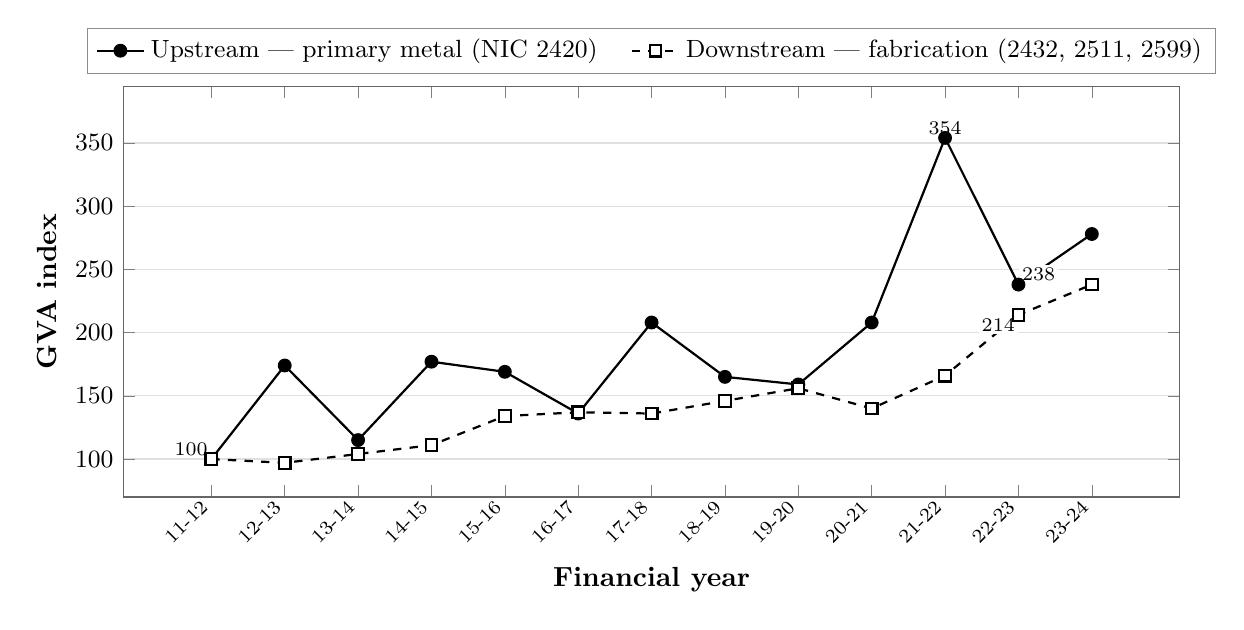
\begin{tikzpicture}
    \begin{axis}[
        asibase,
        height=6.8cm,
        ymin=70, ymax=395,
        ytick={100,150,200,250,300,350},
        ylabel={\textbf{GVA index}},
        xlabel={\textbf{Financial year}},
        symbolic x coords={11-12,12-13,13-14,14-15,15-16,16-17,17-18,18-19,19-20,20-21,21-22,22-23,23-24},
        xtick=data,
        legend columns=2,
        clip=false,
    ]
    \addplot[upstyle]
      coordinates {(11-12,100)(12-13,174)(13-14,115)(14-15,177)(15-16,169)(16-17,136)(17-18,208)(18-19,165)(19-20,159)(20-21,208)(21-22,354)(22-23,238)(23-24,278)};
    \addlegendentry{Upstream --- primary metal (NIC 2420)}
    \addplot[dnstyle]
      coordinates {(11-12,100)(12-13,97)(13-14,104)(14-15,111)(15-16,134)(16-17,137)(17-18,136)(18-19,146)(19-20,156)(20-21,140)(21-22,166)(22-23,214)(23-24,238)};
    \addlegendentry{Downstream --- fabrication (2432, 2511, 2599)}
    \node[font=\scriptsize, fill=white, inner sep=1.1pt, anchor=south] at (axis cs:21-22,354) {354};
    \node[font=\scriptsize, fill=white, inner sep=1.1pt, anchor=south west] at (axis cs:22-23,238) {238};
    \node[font=\scriptsize, fill=white, inner sep=1.1pt, anchor=north east] at (axis cs:22-23,214) {214};
    \node[font=\scriptsize, fill=white, inner sep=1.1pt, anchor=south east] at (axis cs:11-12,100) {100};
    \end{axis}
    \end{tikzpicture}

    \vspace{0.2cm}
    \raggedright
    \small Source: our calculations from ASI All-India summary results.
\end{figure}

The employment arithmetic runs the other way, and it is the heart of the matter. That upstream value added is generated by 170,871 persons engaged; the downstream classes engage \textbf{523,899}. Per head, upstream value added stood at INR 24.97 lakh in 2022--23 against INR 7.95 lakh downstream.

\subsection{Labour Intensity: The Central Finding}

Each rupee of value added created downstream therefore sustains \textbf{3.14 times} more employment than the same rupee created in primary metal. Because this ratio carries most of the section's weight, Figure~\ref{fig:asi_li} shows it for every year rather than for the single year quoted.

\begin{figure}[H]
    \centering
    \captionsetup{font={color=black, normalsize}, justification=centering}
    \caption{Labour intensity of downstream fabrication relative to primary metal}
    \label{fig:asi_li}
    \vspace{0.3cm}

    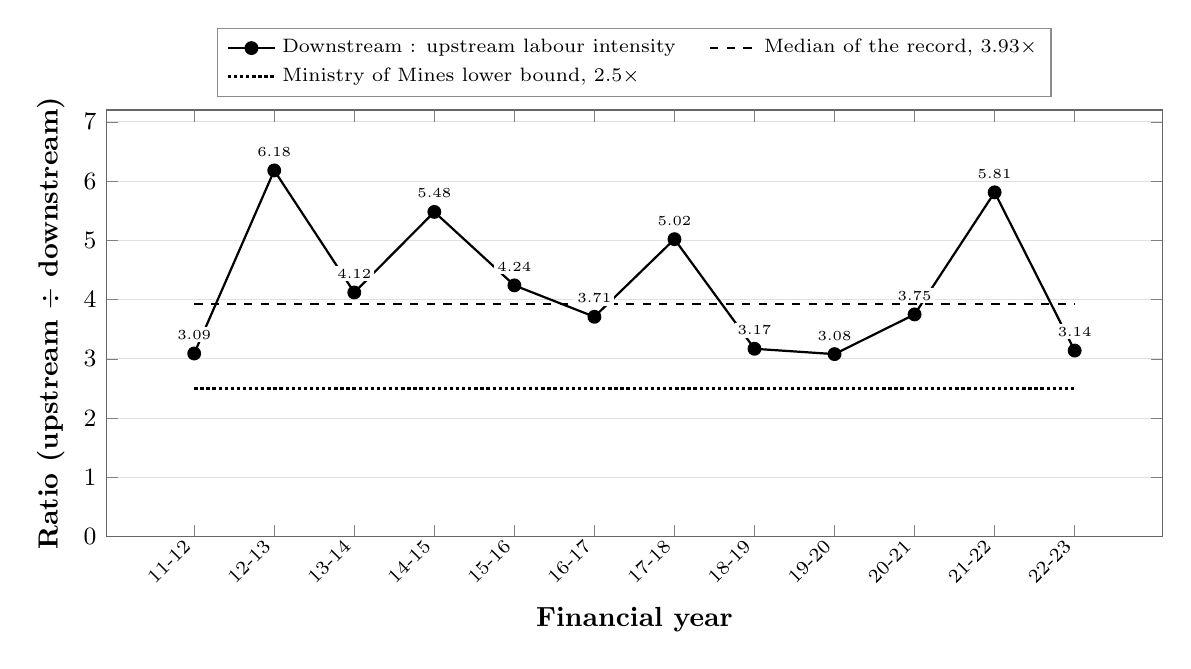
\begin{tikzpicture}
    \begin{axis}[
        asibase,
        height=7.0cm,
        ymin=0, ymax=7.2,
        ytick={0,1,2,3,4,5,6,7},
        ylabel={\textbf{Ratio (upstream $\div$ downstream)}},
        xlabel={\textbf{Financial year}},
        symbolic x coords={11-12,12-13,13-14,14-15,15-16,16-17,17-18,18-19,19-20,20-21,21-22,22-23},
        xtick=data,
        legend columns=2,
        legend style={at={(0.5,1.03)}, anchor=south, draw=black!45, fill=white, font=\scriptsize},
    ]
    \addplot[black, thick, mark=*, mark size=2.1pt, mark options={solid, fill=black},
             nodes near coords, point meta=explicit symbolic,
             every node near coord/.append style={anchor=south, yshift=4pt}]
      coordinates {(11-12,3.09)[3.09](12-13,6.18)[6.18](13-14,4.12)[4.12](14-15,5.48)[5.48](15-16,4.24)[4.24](16-17,3.71)[3.71](17-18,5.02)[5.02](18-19,3.17)[3.17](19-20,3.08)[3.08](20-21,3.75)[3.75](21-22,5.81)[5.81](22-23,3.14)[3.14]};
    \addlegendentry{Downstream : upstream labour intensity}
    \addplot[black, dashed, thick, no marks] coordinates
      {(11-12,3.93)(22-23,3.93)};
    \addlegendentry{Median of the record, 3.93$\times$}
    \addplot[black, densely dotted, very thick, no marks] coordinates
      {(11-12,2.5)(22-23,2.5)};
    \addlegendentry{Ministry of Mines lower bound, 2.5$\times$}
    \end{axis}
    \end{tikzpicture}

    \vspace{0.2cm}
    \raggedright
    \small Source: our calculations from ASI All-India summary results.
\end{figure}

The ratio never falls below \textbf{3.08} and reaches 6.18; its median is \textbf{3.93}. In every one of the twelve years downstream is the more labour-intensive segment, and in every one the ratio exceeds 2.5---the lower bound of the Ministry of Mines' own assessment that downstream activity generates two-and-a-half to three times the employment of primary production \cite{mom_vision2025}. Our estimate corroborates the Ministry's from an independent source and sits at the upper end of its range. The peaks are metal-price years, which raise upstream value added without raising upstream employment; the ratio is therefore lowest in the years least flattering to the argument, and 2022--23, the year quoted throughout, is one of them.

\paragraph{The same finding, per tonne of metal.} Value added is the right denominator for an economic comparison, but a policymaker deciding where a tonne of metal should be converted will ask a blunter question. On that measure the answer is \textbf{41 persons engaged per thousand tonnes upstream against 210 to 262 downstream}, a ratio of \textbf{5.1 to 6.4}. The two normalisations are related exactly, so the segment that is more labour-intensive per rupee is also, and more strongly, more labour-intensive per tonne.\footnote{Derived in Appendix~\ref{app:asi}. Tonnage is not an ASI variable, so this statistic supports the value-added measure rather than replacing it.}

\subsection{Labour Share: Where the Value Added Goes}

Employment counts measure how many people a segment engages, not how much of the value created reaches them. On that second question the divergence is starker, and it depends on no assumption about how persons engaged are counted. In 2022--23 downstream paid out \textbf{38.4 per cent} of gross value added as wages and salaries against \textbf{17.6 per cent} upstream (Figure~\ref{fig:asi_wageshare}).

\begin{figure}[H]
    \centering
    \captionsetup{font={color=black, normalsize}, justification=centering}
    \caption{Wages and salaries as a share of gross value added (per cent)}
    \label{fig:asi_wageshare}
    \vspace{0.3cm}

    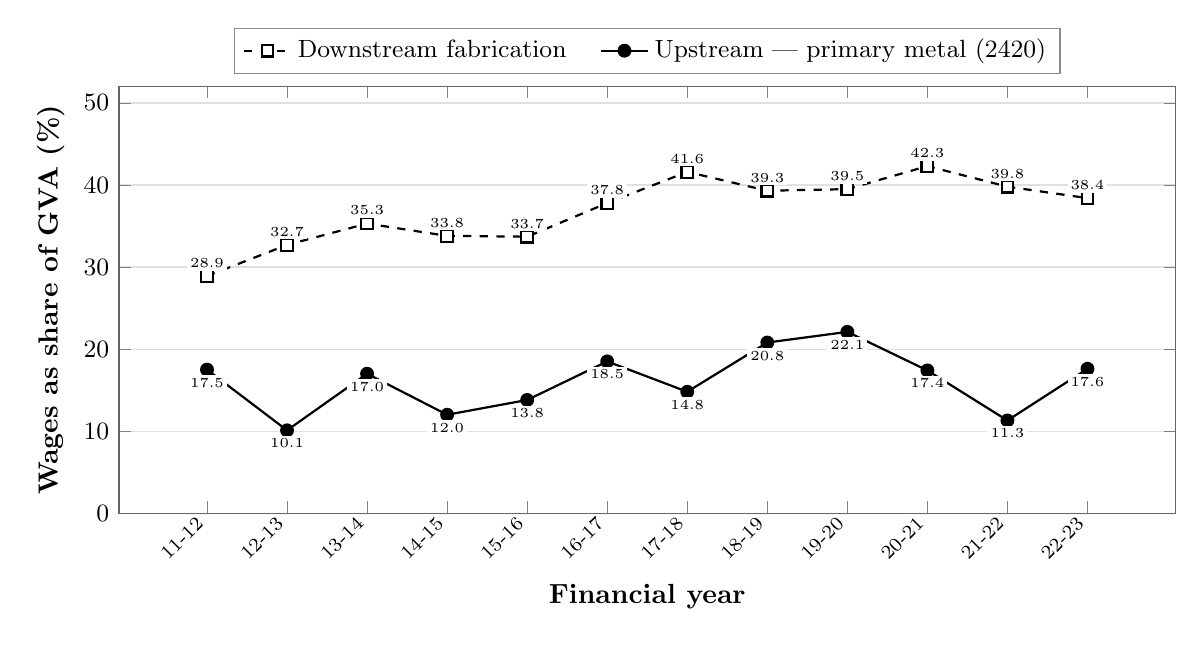
\begin{tikzpicture}
    \begin{axis}[
        asibase,
        height=7.0cm,
        ymin=0, ymax=52,
        ytick={0,10,20,30,40,50},
        ylabel={\textbf{Wages as share of GVA (\%)}},
        xlabel={\textbf{Financial year}},
        symbolic x coords={11-12,12-13,13-14,14-15,15-16,16-17,17-18,18-19,19-20,20-21,21-22,22-23},
        xtick=data,
        legend columns=2,
        nodes near coords, point meta=explicit symbolic,
    ]
    \addplot[dnstyle, every node near coord/.append style={anchor=south, yshift=2pt}]
      coordinates {(11-12,28.9)[28.9](12-13,32.7)[32.7](13-14,35.3)[35.3](14-15,33.8)[33.8](15-16,33.7)[33.7](16-17,37.8)[37.8](17-18,41.6)[41.6](18-19,39.3)[39.3](19-20,39.5)[39.5](20-21,42.3)[42.3](21-22,39.8)[39.8](22-23,38.4)[38.4]};
    \addlegendentry{Downstream fabrication}
    \addplot[upstyle, every node near coord/.append style={anchor=north, yshift=-2pt}]
      coordinates {(11-12,17.5)[17.5](12-13,10.1)[10.1](13-14,17.0)[17.0](14-15,12.0)[12.0](15-16,13.8)[13.8](16-17,18.5)[18.5](17-18,14.8)[14.8](18-19,20.8)[20.8](19-20,22.1)[22.1](20-21,17.4)[17.4](21-22,11.3)[11.3](22-23,17.6)[17.6]};
    \addlegendentry{Upstream --- primary metal (2420)}
    \end{axis}
    \end{tikzpicture}

    \vspace{0.2cm}
    \raggedright
    \small Source: our calculations from ASI All-India summary results.
\end{figure}

The gap is not a single-year artefact: the two series never cross, and the downstream share has \emph{risen} over the period while upstream has oscillated with no trend, its troughs coinciding with the metal-price peaks. A rupee of value added retained downstream delivers roughly \textbf{2.2 times as much to household income} as the same rupee retained upstream---the cleanest single statistic in this section, and the one least exposed to methodological objection.

\subsection{Where the Pressure Falls: Structural Products}

The downstream aggregate conceals a divergence that matters for policy, because it maps onto the effective-protection estimates directly (Figure~\ref{fig:asi_class}).

\begin{figure}[H]
    \centering
    \captionsetup{font={color=black, normalsize}, justification=centering}
    \caption{Gross value added by class, index 2011--12 $=$ 100}
    \label{fig:asi_class}
    \vspace{0.3cm}

    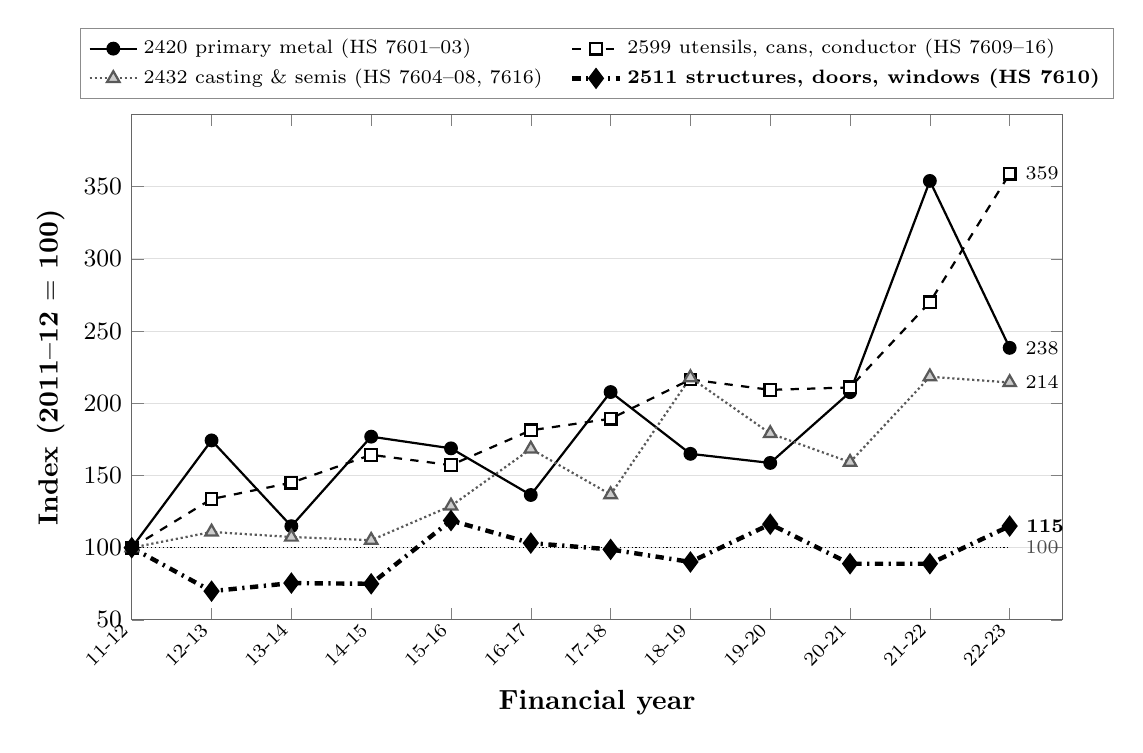
\begin{tikzpicture}
    \begin{axis}[
        asibase,
        height=8.0cm,
        width=13.4cm,
        ymin=50, ymax=400,
        ytick={50,100,150,200,250,300,350},
        ylabel={\textbf{Index (2011--12 $=$ 100)}},
        xlabel={\textbf{Financial year}},
        symbolic x coords={11-12,12-13,13-14,14-15,15-16,16-17,17-18,18-19,19-20,20-21,21-22,22-23},
        xtick=data,
        enlarge x limits={upper, value=0.06},
        legend columns=2,
        legend style={at={(0.5,1.03)}, anchor=south, draw=black!45, fill=white, font=\scriptsize,
                      /tikz/every even column/.append style={column sep=8pt}},
        clip=false,
    ]
    \addplot[black, densely dotted, no marks, forget plot] coordinates {(11-12,100)(22-23,100)};
    \addplot[upstyle]
      coordinates {(11-12,100.0)(12-13,174.3)(13-14,114.9)(14-15,176.9)(15-16,168.8)(16-17,136.5)(17-18,207.8)(18-19,165.0)(19-20,158.7)(20-21,207.7)(21-22,354.0)(22-23,238.4)};
    \addlegendentry{2420 primary metal (HS 7601--03)}
    \addplot[dnstyle]
      coordinates {(11-12,100.0)(12-13,133.7)(13-14,145.0)(14-15,164.3)(15-16,157.2)(16-17,181.3)(17-18,189.3)(18-19,216.5)(19-20,209.3)(20-21,211.0)(21-22,270.0)(22-23,359.0)};
    \addlegendentry{2599 utensils, cans, conductor (HS 7609--16)}
    \addplot[altA]
      coordinates {(11-12,100.0)(12-13,110.9)(13-14,107.4)(14-15,105.2)(15-16,128.9)(16-17,168.4)(17-18,136.8)(18-19,217.8)(19-20,179.1)(20-21,159.2)(21-22,218.4)(22-23,214.4)};
    \addlegendentry{2432 casting \& semis (HS 7604--08, 7616)}
    \addplot[altB, ultra thick, mark options={solid, fill=black}]
      coordinates {(11-12,100.0)(12-13,69.9)(13-14,75.5)(14-15,75.0)(15-16,118.8)(16-17,103.2)(17-18,98.8)(18-19,90.1)(19-20,116.3)(20-21,88.9)(21-22,88.9)(22-23,115.0)};
    \addlegendentry{\textbf{2511 structures, doors, windows (HS 7610)}}

    % direct end-of-series labels
    \node[font=\scriptsize, anchor=west] at (axis cs:22-23,238.4) {\;238};
    \node[font=\scriptsize, anchor=west] at (axis cs:22-23,359.0) {\;359};
    \node[font=\scriptsize, anchor=west] at (axis cs:22-23,214.4) {\;214};
    \node[font=\scriptsize\bfseries, anchor=west] at (axis cs:22-23,115.0) {\;115};
    \node[font=\scriptsize, anchor=west, black!70] at (axis cs:22-23,100) {\;100};
    \end{axis}
    \end{tikzpicture}

    \vspace{0.2cm}
    \raggedright
    \small Source: our calculations from ASI All-India summary results.
\end{figure}

\textbf{Structural metal products (NIC~2511)}---the class that makes HS~7610 aluminium frameworks, doors, windows and fa\c{c}ades---grew gross value added by \textbf{15.0 per cent} over eleven nominal years, and by 19.4 per cent on the three-year-average basis. Against any plausible measure of cumulative inflation that is a deep real contraction. Its persons engaged rose 0.2 per cent and \emph{fell} 5.9 per cent between the three-year endpoints; its contract workforce fell 1.1 per cent; its estimated tax contribution declined 16.1 per cent. Every indicator points the same way.

This is not an arbitrary class to find under pressure. HS~7610 carries among the highest disprotection in the entire ERP table---by 2024--25, negative effective protection against Malaysia, Korea, Japan and Thailand alike, against a non-preferential benchmark of $+0.51$. The single ASI class most exposed to duty-free finished imports is the single ASI class that has not grown.

\begin{table}[H]
    \centering
    \caption{Percentage change by NIC class, 2011--12 to 2022--23 (nominal)}
    \label{tab:asi_growth}
    \resizebox{\textwidth}{!}{
    \begin{tabular}{llrrrrrr}
        \toprule
        \textbf{NIC class} & \textbf{HS lines} & \textbf{GVA} & \textbf{Persons} & \textbf{Workers} & \textbf{Contract} & \textbf{Wages} & \textbf{Tax} \\
        \midrule
        \multicolumn{8}{l}{\textit{Upstream --- the protected input}} \\
        2420 Primary metal and semis & 7601--7603 & $+138.4$ & $+39.5$ & $+48.7$ & $+100.0$ & $+139.6$ & $+181.6$ \\
        \midrule
        \multicolumn{8}{l}{\textit{Downstream --- the ERP basket}} \\
        2432 Casting of non-ferrous metals & 7604--08, 7616 & $+114.4$ & $+11.9$ & $+14.8$ & $+28.6$ & $+153.6$ & $+196.8$ \\
        2511 Structural metal products & 7610 & \textbf{+15.0} & \textbf{+0.2} & $+0.3$ & $-1.1$ & $+102.6$ & \textbf{--16.1} \\
        2599 Other fabricated metal products & 7609, 7612--16 & $+259.0$ & $+50.9$ & $+49.8$ & $+16.0$ & $+263.6$ & $+412.4$ \\
        \midrule
        \textbf{Upstream total} & & \textbf{+138.4} & \textbf{+39.5} & \textbf{+48.7} & \textbf{+100.0} & \textbf{+139.6} & \textbf{+181.6} \\
        \textbf{Downstream total} & & \textbf{+114.5} & \textbf{+27.4} & \textbf{+27.1} & \textbf{+9.0} & \textbf{+184.5} & \textbf{+110.1} \\
        \bottomrule
    \end{tabular}
    }

    \vspace{0.2cm}
    \raggedright
    \small Source: our calculations from ASI All-India summary results.
\end{table}

\subsection{Employment Composition}

Chaurey \cite{chaurey2015} shows that Indian manufacturers use contract labour as their margin of flexibility, because permanent workers are difficult to adjust under employment protection legislation. The two segments have used that margin in opposite directions (Figure~\ref{fig:asi_contract}). Upstream, the contract workforce \textbf{doubled}, from 37,228 to 74,449, and its share of total workers climbed from 40.2 to \textbf{54.1 per cent}. Downstream, contract employment rose 9.0 per cent and the share \emph{fell}, from 47.6 to \textbf{40.9 per cent}.

\begin{figure}[H]
    \centering
    \captionsetup{font={color=black, normalsize}, justification=centering}
    \caption{Workers employed through contractors as a share of total workers (per cent)}
    \label{fig:asi_contract}
    \vspace{0.3cm}

    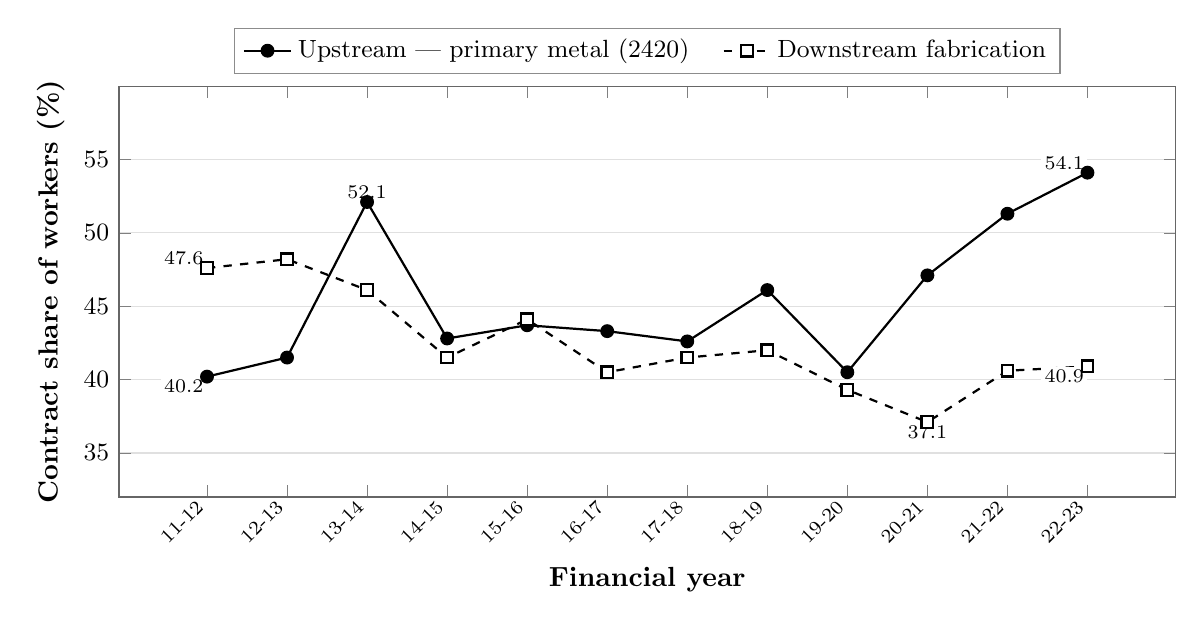
\begin{tikzpicture}
    \begin{axis}[
        asibase,
        height=6.8cm,
        ymin=32, ymax=60,
        ytick={35,40,45,50,55},
        ylabel={\textbf{Contract share of workers (\%)}},
        xlabel={\textbf{Financial year}},
        symbolic x coords={11-12,12-13,13-14,14-15,15-16,16-17,17-18,18-19,19-20,20-21,21-22,22-23},
        xtick=data,
        legend columns=2,
        clip=false,
    ]
    \addplot[upstyle]
      coordinates {(11-12,40.2)(12-13,41.5)(13-14,52.1)(14-15,42.8)(15-16,43.7)(16-17,43.3)(17-18,42.6)(18-19,46.1)(19-20,40.5)(20-21,47.1)(21-22,51.3)(22-23,54.1)};
    \addlegendentry{Upstream --- primary metal (2420)}
    \addplot[dnstyle]
      coordinates {(11-12,47.6)(12-13,48.2)(13-14,46.1)(14-15,41.5)(15-16,44.1)(16-17,40.5)(17-18,41.5)(18-19,42.0)(19-20,39.3)(20-21,37.1)(21-22,40.6)(22-23,40.9)};
    \addlegendentry{Downstream fabrication}
    \node[font=\scriptsize, fill=white, inner sep=1.1pt, anchor=north east] at (axis cs:11-12,40.2) {40.2};
    \node[font=\scriptsize, fill=white, inner sep=1.1pt, anchor=south east] at (axis cs:11-12,47.6) {47.6};
    \node[font=\scriptsize, fill=white, inner sep=1.1pt, anchor=south] at (axis cs:13-14,52.1) {52.1};
    \node[font=\scriptsize, fill=white, inner sep=1.1pt, anchor=north] at (axis cs:20-21,37.1) {37.1};
    \node[font=\scriptsize, fill=white, inner sep=1.1pt, anchor=south east] at (axis cs:22-23,54.1) {54.1};
    \node[font=\scriptsize, fill=white, inner sep=1.1pt, anchor=north east] at (axis cs:22-23,40.9) {40.9};
    \end{axis}
    \end{tikzpicture}

    \vspace{0.2cm}
    \raggedright
    \small Source: our calculations from ASI All-India summary results.
\end{figure}

The falling downstream share is not improving job quality; it is the signature of a segment that has stopped hiring. Downstream nominal value added more than doubled while its flexible workforce grew nine per cent---the segment is running existing capacity harder rather than adding to it. Upstream, by contrast, expanded employment and casualised it. A segment under sustained margin pressure does not, on this evidence, shed workers so much as stop taking them on, and foregone employment appears in no redundancy statistic.

\subsection{Corporate Tax: Employment Yield and Revenue Stability}

The ASI does not publish tax paid, so corporate tax here is an \emph{estimate} of the tax base attributable to each segment rather than a record of receipts. On levels, upstream is ahead: an estimated INR 4,411 crore in 2022--23 against INR 3,473 crore downstream. Levels are the wrong test for a tariff decision, for two reasons.

First, the employment attached to each rupee differs by nearly a factor of four. The downstream classes support \textbf{151 persons engaged per crore} of estimated corporate tax against \textbf{39} upstream, and the ordering holds in all twelve years without the gap ever falling below a factor of two (Figure~\ref{fig:asi_yield}).

\begin{figure}[H]
    \centering
    \captionsetup{font={color=black, normalsize}, justification=centering}
    \caption{Persons engaged per INR crore of estimated corporate tax}
    \label{fig:asi_yield}
    \vspace{0.3cm}

    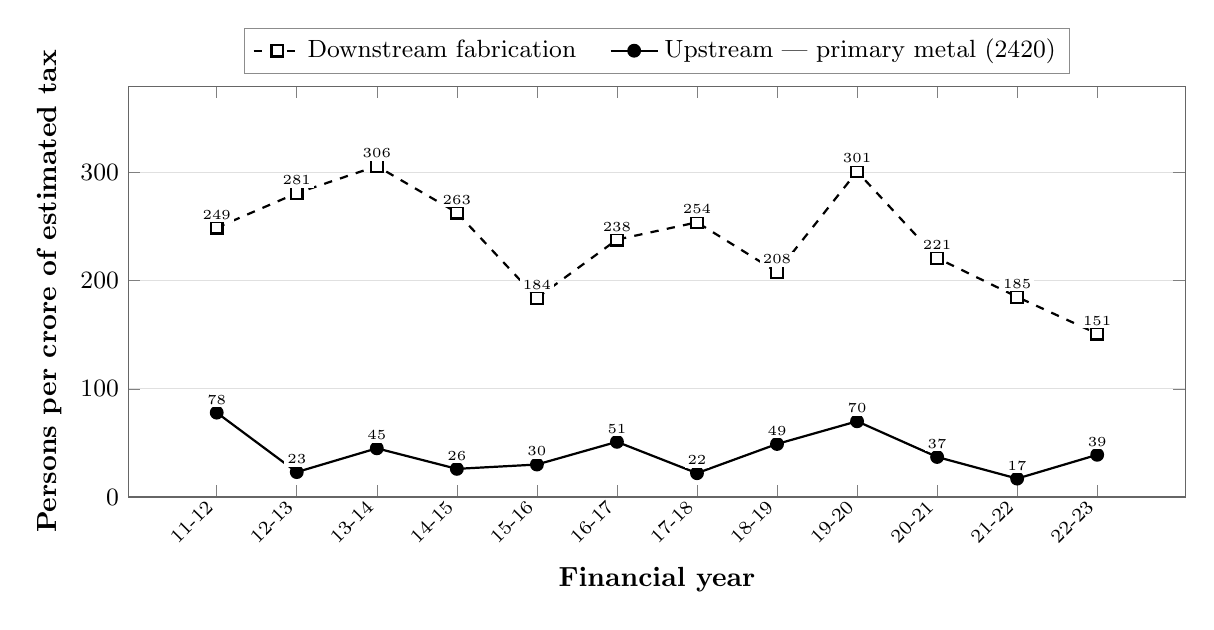
\begin{tikzpicture}
    \begin{axis}[
        asibase,
        height=6.8cm,
        ymin=0, ymax=380,
        ytick={0,100,200,300},
        ylabel={\textbf{Persons per crore of estimated tax}},
        xlabel={\textbf{Financial year}},
        symbolic x coords={11-12,12-13,13-14,14-15,15-16,16-17,17-18,18-19,19-20,20-21,21-22,22-23},
        xtick=data,
        legend columns=2,
        nodes near coords, point meta=explicit symbolic,
    ]
    \addplot[dnstyle, every node near coord/.append style={anchor=south, yshift=2pt}]
      coordinates {(11-12,249)[249](12-13,281)[281](13-14,306)[306](14-15,263)[263](15-16,184)[184](16-17,238)[238](17-18,254)[254](18-19,208)[208](19-20,301)[301](20-21,221)[221](21-22,185)[185](22-23,151)[151]};
    \addlegendentry{Downstream fabrication}
    % Both series labelled above: the gap between them is wide enough that
    % upward labels never collide, and downward ones would hit the axis.
    \addplot[upstyle, every node near coord/.append style={anchor=south, yshift=2pt}]
      coordinates {(11-12,78)[78](12-13,23)[23](13-14,45)[45](14-15,26)[26](15-16,30)[30](16-17,51)[51](17-18,22)[22](18-19,49)[49](19-20,70)[70](20-21,37)[37](21-22,17)[17](22-23,39)[39]};
    \addlegendentry{Upstream --- primary metal (2420)}
    \end{axis}
    \end{tikzpicture}

    \vspace{0.2cm}
    \raggedright
    \small Source: our calculations from ASI All-India summary results.
\end{figure}

Second, the two revenue streams are of different quality. Upstream tax has run from INR 1,567 crore to INR 8,996 crore at the 2021--22 price peak and back to INR 4,411 crore a year later; downstream tax has risen in a near-monotone line from INR 1,653 crore to INR 3,473 crore. The underlying volatility runs the same way: the standard deviation of year-on-year log growth in value added is \textbf{0.373} upstream against \textbf{0.105} downstream, so the protected node's value added is \textbf{3.6 times as volatile}. Rationalising the duty on primary aluminium therefore trades a \emph{cyclical} revenue stream, thinly attached to employment, for relief to a segment on which roughly four times as many livelihoods depend per rupee of tax at stake.

\paragraph{The transmission mechanism, and its magnitude.} Bought-in inputs account for \textbf{83.1 per cent} of downstream output value---four-fifths of every rupee of turnover is purchased material, overwhelmingly metal bought at import-parity prices set by a duty the fabricator cannot avoid and, on the evidence of Section~\ref{sec:erp}, cannot pass into an output price that competes with duty-free finished imports. Because value added is what remains after inputs, the ratio of the two---\textbf{4.91}---is the factor by which any proportional change in input cost is amplified by the time it reaches value added. Where metal is 60 per cent of the downstream input bill, a one per cent rise in the metal price removes about \textbf{3 per cent} of downstream value added and the 7.5 per cent duty something over a fifth of it; upstream the figure is nil, because a smelter does not buy the metal it makes.\footnote{Derivation and the full range in Appendix~\ref{app:asi}.} This is Corden's arithmetic in its plainest form \cite{corden1966}: an input-price wedge of that size cannot be a marginal factor in downstream margins.

\subsection{The Two Segments at a Glance}

Figure~\ref{fig:asi_summary} collects the four measures on which this section rests. Each is expressed as a multiple so the four are comparable, and each is drawn from a different part of the ASI schedule---value added and employment, wages, corporate tax, and the variance of value added. They are not four versions of one statistic.

\begin{figure}[H]
    \centering
    \captionsetup{font={color=black, normalsize}, justification=centering}
    \caption{How far the two segments differ, 2022--23 (parity $=$ 1.0$\times$)}
    \label{fig:asi_summary}
    \vspace{0.3cm}

    \begin{tikzpicture}
    \begin{axis}[
        xbar,
        width=12.6cm, height=6.0cm,
        bar width=13pt,
        xmin=0, xmax=4.6,
        xtick={0,1,2,3,4},
        xlabel={\textbf{Multiple}},
        symbolic y coords={Volatility,Jobs per rupee of estimated tax,Labour share of value added,Labour intensity},
        ytick=data,
        y tick label style={font=\small, align=right},
        tick label style={font=\small},
        xmajorgrids=true, major grid style={black!12},
        axis line style={black!60},
        nodes near coords={\pgfmathprintnumber[precision=2, fixed, fixed zerofill]{\pgfplotspointmeta}$\times$},
        every node near coord/.append style={font=\small\bfseries, anchor=west},
        enlarge y limits=0.2,
    ]
    \addplot[fill=g5, draw=black, line width=0.6pt]
      coordinates {(3.14,Labour intensity) (2.18,Labour share of value added)
                   (3.89,Jobs per rupee of estimated tax) (3.57,Volatility)};
    \draw[black, densely dashed, thick] (axis cs:1,Volatility) -- (axis cs:1,Labour intensity);
    \end{axis}
    \end{tikzpicture}

    \vspace{0.2cm}
    \raggedright
    \small Source: our calculations from ASI All-India summary results.
\end{figure}

The first three favour downstream on employment and household-income grounds; the fourth favours it on revenue stability, since it is \emph{upstream} value added that is the more volatile. Every claim above was tested against the obvious objections---choice of year and base year, the exclusion of any single class, the placement of semi-fabrication, the width of the downstream basket, and the possibility that the classes should be scaled by their aluminium content. None changes a sign, and the largest moves the labour-intensity ratio only from 3.14 to 2.61. The tests and the assumptions they probe are in Appendix~\ref{app:asi}.

